\documentclass[12pt, a4paper]{article}

    \usepackage[spanish, es-tabla]{babel}
    \selectlanguage{spanish}
    \usepackage[utf8]{inputenc}
    \usepackage{listings, xcolor}
    \usepackage{graphicx}
    \usepackage[hidelinks]{hyperref}

    \graphicspath{ {images/} }
    
    \lstset{
        basicstyle={\small\ttfamily},
        numbers=none,
        breaklines=true,
        breakatwhitespace=true,
        string=[s]{"}{"},
        stringstyle=\color{blue},
        comment=[l]{:},
        commentstyle=\color{black}
    }

    \begin{document}

        \title{% 
            \huge \textbf{Pipeline para el Análisis en Tiempo Real de datos IoT} \\ \bigskip
            \LARGE Trabajo de Investigación \\ \medskip
            \Large Internet de las Cosas en el Contexto de Big Data\\ \smallskip
            \normalsize Máster en Tecnologías de Análisis de Datos Masivos: Big Data
        }
        \author{Adrián Miralles Palazón}
        \date{\today}
        \maketitle

        \begin{figure}[ht]
            \centerline{
\includegraphics[]{logo}}
        \end{figure}

        \clearpage
        \tableofcontents
        
        \clearpage
        \section{Introducción}

        \paragraph{}
        El ecosistema de tecnologías desarrolladas para el análisis inteligente de datos producidos por dispositivos o sensores conectados, Internet de las Cosas (IoT), se encuentra en una fase de maduración e implantación en numerosas industrias. Casi todos los dispositivos que se utilizan se están convirtiendo en dispositivos inteligentes que están continuamente generando datos sobre parámetros internos o del medio que los rodea.

        \paragraph{}
        La recolección, el preprocesamiento, el almacenamiento y el análisis posterior de estos datos debe ser establecido mediante un procedimiento que permita la obtención de resultados clave para el dominio de aplicación del problema a solventar. Este procedimiento se conoce como \textit{data pipeline} por los analistas de datos.

        \paragraph{}
        En cada una de estas fases es posible la utilización de tecnologías tradicionales. Sin embargo, las características que suelen tener los escenarios IoT provocan que sea necesario la utilización de tecnologías que han sido desarrolladas específicamente para entornos de este tipo. Entre estas características destacan la localización distribuida de los dispositivos que poseen los sensores, las ingentes cantidades de información que estos generan y la escasa capacidad de cómputo que tienen estos dispositivos.


        \section{Motivación y objetivos}

        \paragraph{}
        Estar al día de todas las tecnologías que surgen para la realización de todas las tareas relacionadas con el proceso de extracción, procesamiento y análisis de los datos es una de las labores más complicadas a las que se enfrenta un profesional de este campo.

        \paragraph{}
        Este hecho se convierte en un problema para titulaciones especializadas en este sector como el título de Máster en Tecnologías de Análisis de Datos Masivos: BIG DATA en el que se enmarca este trabajo. Resulta prácticamente imposible que el contenido que forma parte del plan de estudios de estas titulaciones cumpla con las espectativas del alumnado ya que siempre quedarán temas y tecnologías por tratar.

        \paragraph{}
        No obstante, este tipo de trabajo deberían ser una opción extraordianaria para los alumnos para llevar a cabo este tipo de tareas de profundización en algunos temas o tecnologías.

        \paragraph{}
        Bajo este argumento surge la idea de este trabajo en el que se establece como objetivo llevar a cabo una implementación práctica de un \textit{data pipeline} utilizando tecnologías que no hayan sido puestas en práctica en ninguna de las asignaturas de la titulación.

        \paragraph{}
        Para ello, será necesario estudiar las alternativas existentes en cada uno las etapas existentes para realizar la sensorización, extracción de los datos, realizar el procesamiento de los mismos y el almacenamiento para el posterior análisis de toda la información. La selección de una tecnología no sólo deberá estar marcada por adecuarse a las tareas que se requieren sino que también deberá cumplir la condición de no haber sido estudiada previamente.

        \section{Estado de arte}

        \paragraph{}
        Cumpliendo con las restricciones establecidas en los objetivos planteados en la sección anterior, se han seleccionado las siguientes herramientas o tecnologías para la creación del \textit{data pipeline}. 
        
        \paragraph{}
        Para la sensorización, se utilizará un dispositivo de bajo coste conocido como Raspberry Pi \cite{raspberry}. Para la comunicación de estos dispositivos con una plataforma donde poder agregar la información se utilizan dos tecnologías: MQTT \cite{mqtt} es un protocolo que facilita la comunicación con los dispositivos situados de forma distribuida y Apache Kafka \cite{kafka} es una plataforma que permite escalar horizontalmente de forma muy sencilla el procesamiento de los datos para su almacenamiento. Con respecto al almacenamiento, se ha seleccionado InfluxDB \cite{influx}, una base de datos de código abierto que está optimizada para el almacenamiento rápido y de alta diponibilidad de series temprales. Finalmente, se utiliza Grafana \cite{grafana} para la creación de una serie de cuados de mando que faciliten el análisis y visualización de los datos que generan los dispositivos.

        \paragraph{}
        A continuación, se incluye una breve descripción teórica de cada una de los dispositivos, herramientas o tecnologías que se han seleccionado.

        \subsection{Raspberry Pi}
        
        \paragraph{}
        La Raspberry Pi es un ordenador pequeño y de bajo coste que tiene como objetivo poner el poder de la computación en manos de gente de cualquier parte del mundo. Sus características lo han convertido, junto a Arduino, en una de las piezas angulares de la gran mayoría de proyectos de sensorización.

        \paragraph{}
        La presencia de pines GPIO \cite{gpio} es precisamente la característica que más influencia tiene en este hecho. Estos pines son los que permiten la conexión de los distintos sensores. Un aspecto relevante en este aspecto es que la Raspberry Pi no posee pines analógicos por lo que solo será posible utilizar sensores puramente digitales.

        \paragraph{}
        Del mismo modo, existen distintos modelos de Raspberry Pi que varían sus especificaciones. Entre éstas es necesario destacar las distintas herramientas para la conectividad que presenta. Por ejemplo, existen modelos que poseen módulos para la conexión con tecnologías inalámbricas y otros que no. Aunque esta característica no va a ser imprescindible para el escenario de prueba pero si que es una especificación que habría que tener muy en cuenta para un eventual despliegue real.

        \subsection{Message Queuing Telemetry Transport (MQTT)}
        
        \paragraph{}
        MQTT es un protocolo de intercambio de mensajes extremadamente liviano y sencillo. Se basa en un modelo de publicación y subscripción. Ha sido diseñado para dispositivos con recursos limitados, que disponen de poco ancho de banda para comunicarse, con latencias muy altas y sobre redes poco confiables.

        \paragraph{}
        Los principios que se utilizaron para su diseño fueron minimizar el ancho de banda necesario y los recursos que el dispositivo debería reservar. Todo esto sin obviar la necesidad de intentar asegurar algún grado de confianza en la entrega. Todos estos principios lo han convertido en una de las alternativas más usadas en entornos IoT donde la bateria y el ancho de banda de los dispositivos es uno de los factores más relevantes a la hora de elegir un protocolo.

        \paragraph{}
        MQTT es un protocolo que se utiliza sobre la pila de protocolos TCP/IP \cite{rfc793} frente a otros protocolos como COAP \cite{rfc7252} que utiliza UDP \cite{rfc768}. Sin embargo, existe una versión MQTT-SN que pretende eliminar esta restricción y extender el uso de MQTT más allá de la infraestructura TCP/IP.

        \paragraph{}
        Este protocolo define las entidades de \textit{client} y \textit{broker}. Los clientes se conectan al broker y se suscriben a diferentes \textit{topics}, esto es, tipos de mensajes que desean recibir. Los clientes también pueden publicar mensajes en un determinado topic comunicándoselo al broker. Por tanto, el broker es la figura que trata de comunicar a los dispositivos que se suscriben a un topic con los que publican mensajes sobre ese topic.

        \paragraph{}
        Los topics son organizados de forma jerárquica para permitir la agregación de posibles tipos de mensajes relacionados. Para ello se utiliza una nomenclatura similar a la utilizada en los sistemas de ficheros convencionales. Por ejemplo, el topic \textit{UMU/FacInformatica/Lab24/temperature} representaría un tipo de mensajes que contienen la temperatura del laboratorio 2.4 de la Facultad de Informática de la UMU. Sin embargo, es posible recibir este tipo de mensajes con una suscripción al topic \textit{UMU/FacInformatica} para facilitar la agregación.

        \subsection{Apache Kafka}
        
        \paragraph{}
        Apache Kafka es una plataforma para la gestión de streams de datos en tiempo real de forma distribuida. Se utiliza para construir \textit{data pipelines} que sean horizontalmente escalables y tolerantes a fallos. Es una plataforma que esta siendo utilizada en producción por grandes compañías.

        \paragraph{}
        Su funcionamiento se basa en los mismos conceptos que MQTT, es decir, utiliza un esquema de publicación y suscripción a diferentes streams asociados a un tema. Sin embargo, sus características son diferentes. Esta plataforma se encarga de almacenar los streams de datos para que sean tolerantes a fallos. Para ello, se suele ejecutar sobre un cluster de servidores que almacenan los distintos registros de datos en topics. 

        \paragraph{}
        La arquitectura de Kafka es más compleja que la que propone MQTT pese a seguir un esquema similar. El cluster de servidores sobre el que se ejecuta mantiene una serie de particiones en las que se replica la información entre los distintos servidores. Además, Kafka separa las entidades de los clientes de la plataforma entre los \textit{Producers} que son los encargados de generar los datos que se publican en un determinado \textit{topic} asignando cada registro de datos a una determinada partición. Por otro lado, se encuentra la figura de los \textit{Consumers}, que se encuentran agregados en grupos que se suscriben a un determinado topic. Un registro de datos que se publica a un topic es entregado sólo a un grupo de Consumers para que lo procese. Cada grupo debe gestionar los datos que recibe para que sean procesados de forma balanceada entre los distintos Consumers.

        \paragraph{}
        Este tipo de plataformas está siendo utilizada principalmente para la construcción de \textit{data pipelines} que necesitan funcionar en tiempo real para proporcionar confianza en la distribución de los datos entre unos sistemas y otros.

        \paragraph{}
        La utilización de una plataforma de este tipo para un escenario de prueba puede parecer forzada puesto que la cantidad de datos que se generan no es considerable. Es lógico creer que un sencillo programa que se suscribe a los distintos brokers MQTT en los que publican los mensajes los dispositivos y que almacena esta información en una base de datos. Esto sería correcto si se piensa en un escenario pequeño. No obstante, es conveniente realizar el ejercicio de pensar en cómo escalaría este sistema si se necesita monitorizar datos emitidos por todos los dispositivos móviles del planeta. Este sencillo programa no podría ser ejecutado en ningún ordenador. Por este motivo, es necesario recurrir a plataformas como Apache Kafka que permiten escalar horizontalmente de forma sencilla este tipo de sistemas.
        
        \subsection{InfluxDB}

        \paragraph{}
        InfluxDB es una base datos de código abierto desarrollada por InfluxData que ha sido desarrollada y optimizada para la gestión de datos pertenecientes a series temporales. Sus características la han convertido en un referente para tareas de monitorización, gestión de métricas o análsis de datos procedentes de sensores IoT.

        \paragraph{}
        Ha sido construida para poder ser escalada utilizando clusters de servidores que garanticen la alta disponibilidad y eliminen la existencia de un punto único de fallo. Para su gestión proporciona un lenguaje similar a SQL con funciones específicas para la consulta de datos que suelen estar compuestos por medidas, series o puntos.

        \subsection{Grafana}

        \paragraph{}
        Grafana es una herramienta \textit{open-source} desarrollada para facilitar la visualización y análisis de datos procedentes de distintas métricas. Se centra en el análisis de datos procedentes de series temporales ofreciendo herramientas que faciliten el tratamiento de los mismos.

        \paragraph{}
        Ofrece compatibilidad con la gran mayoría de bases de datos que están siendo utilizadas actualmente para almacenar este tipo de información como pueden ser InfluxDB, Graphite, Prometheus o Elasticsearch.

        \paragraph{}
        Sus herramientas se basan en la construcción de cuadros de mando o dashboards que permiten administrar toda la información disponible en de forma más cómoda. Estos dashboards no se limitan a la administación tradicional sino que se ofrecen herramientas que permiten compartir mediante enlaces la información de los mismos con distintos usuarios así como la creación de instantáneas fácilmente compartibles.

        \section{Diseño de solución}

        \paragraph{}
        Para llevar a cabo un \textit{data pipeline} que nos permita poner en marcha todas las tecnologías descritas en el apartado anterior, es necesario, definir un escenario de aplicación. Este escenario consiste en una serie de dispositivos situados en cada una de las estancias de los edificios públicos de la Universidad de Murcia. El objetivo de estos dispositivos sería obtener información con distintos sensores sobre la temperatura, humedad, luminosidad, niveles de C02 y el ruido. El objetivo del \textit{data pipeline} sería agrupar toda la información que registran los dispositivos para que pueda ser analizada.
        
        \paragraph{}
        Para llevar este escenario a la práctica es necesario tener en cuenta que no es posible realizar un despliegue de estas características. Tampoco es posible acceder a los datos de dispositivos que ya hayan podido ser desplegados previamente. No obstante, se pretende realizar una simulación con los recursos disponibles que permita entender las dimensiones del mismo.

        \subsection{Entidades}

        \paragraph{}
        Dejando el escenario de aplicación a un lado, en esta sección, se trata de plantear las distintas figuras que deben aparecer en un \textit{data pipeline} que utiliza las tecnologías anteriores y cómo éstas deben interactuar entre ellas. La figura \ref{fig-design} muestra las entidades que se han definido siguiendo una arquitectura similar a la de referencia comentada en clase.

        \begin{figure}[ht]
            \centerline{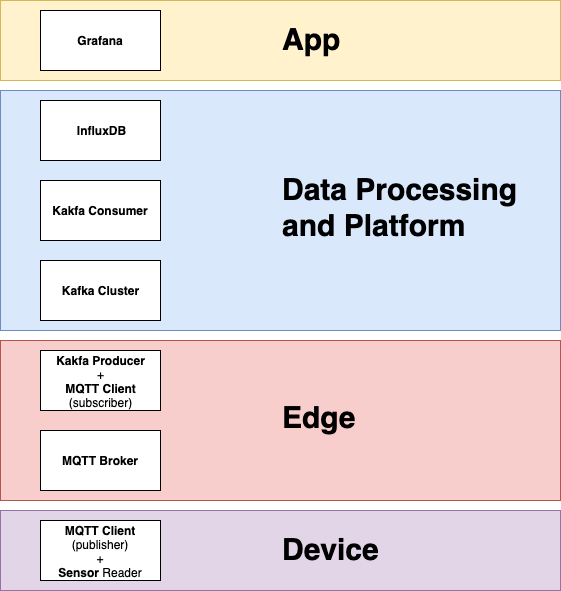
\includegraphics[width=0.6\paperwidth]{design}}
            \caption{Entidades del \textit{data pipeline} propuesto.}
            \label{fig-design}
        \end{figure}

        \subsubsection{Sensor Reader + MQTT Client (publisher)}

        \paragraph{}
        Realizando un recorrido entre las entidades que intervienen desde la generación de los datos hasta su análisis final, es necesario comenzar por la figura encargada de leer los datos de los distintos sensores.

        \paragraph{}
        Estos datos deben ser publicados utilizando el protocolo MQTT en un MQTT Broker. Para ello, es necesario que esta entidad actue como un MQTT Client en el rol de \textit{publisher}, es decir, actua realizando un envío de los datos en el topic que corresponda a las medidas de cada sensor.

        \paragraph{}
        La jerarquía que se utiliza para los distintos topics MQTT sigue el esquema \textbf{UNIVERSIDAD/EDIFICIO/ESTANCIA/SENSOR}. Este esquema permite que los topics puedan ser agregados como se comentó en la sección perteneciente a esta tecnología.

        \subsubsection{MQTT Broker}

        \paragraph{}
        Esta entidad es la encargada de comunicar a los distintos MQTT Client del escenario. Su objetivo principal es que los mensajes que los MQTT Client publican sobre un topic, llegue a los MQTT Client que se han suscrito a dicho topic.

        \paragraph{}
        En principio, se considera que esta entidad no debe ser personalizada para nuestro escenario por lo que cualquier implementación de un MQTT Broker debería servir para realizar las tareas de esta entidad. Más adelante, se analiza la opción que se ha considerado.

        \subsubsection{MQTT Client (subscriber) + Kafka Producer}

        \paragraph{}
        El siguiente eslabón es una entidad cuyo objetivo es recopilar todos las datos recogidos por un MQTT Broker sobre un topic, es decir, todas las mediciones publicadas por los dispositivos. Para ello, toma el papel de MQTT Client en rol de \textit{subscriber} para realizar una suscripción a los topic del MQTT Broker que contienen la información que le intersa.

        \paragraph{}
        Del mismo modo, esta entidad debe procesar los datos para generar un stream de información que pueda ser enviado al Kafka Cluster. Para ello, actúa como un Kafka Producer. También es interesante destacar que en esta entidad, se podría realizar algunas labores de preprocesamiento de los datos como podría ser tratar de eliminar aquellas mediciones que contienen datos erróneos.

        \subsubsection{Kafka Cluster}

        \paragraph{}
        La entidad más compleja de todo el \textit{data pipeline} definido es, sin ninguna duda, este cluster. La unidad sobre la que se articula la plataforma Kafka suele estar formada por un conjunto de servidores que son coordinados para sincronizar el procesamiento entre los Producers y los Consumers de los streams de información. Este conjunto de servidores deben garantizar que exista tolerancia a fallos y que no exista pérdida de información.

        \paragraph{}
        Diseñar una arquitectura para este cluster queda fuera del ámbito de este trabajo. Por tanto, se ha optado por considerar que este cluster está formado por un sólo servidor que debería ofrecer todas las garantías que ofrece la plataforma Kafka.

        \subsubsection{Kafka Consumer}

        \paragraph{}
        Como consecuencia de la arquitectura que propone la plataforma Apache Kafka surge esta entidad en la que se procesa de forma distribuida los streams de datos generados. El objetivo de esta entidad es recoger toda la información para almacenarla en bases de datos.

        \paragraph{}
        Así pues, este tipo de figura deberá actuar como un Kafka Consumer que recoja los datos del Kafka Cluster. Estos datos los deberá almacenar en la base de datos que hemos seleccionado, es decir, InfluxDB. Para representar la información, este tipo de base de datos utiliza una estructura formateada como un documento JSON.

        \subsubsection{InfluxDB}

        \paragraph{}
        El Kafka Consumer debe almacenar la información en una base datos. Como se ha visto, se ha seleccionado InfluxDB como soporte de almacenamiento. Esta plataforma puede ser desplegada en un servidor de forma sencilla y ofrece soporte para ofrecer escalabilidad horizontal. No obstante, el alcance de este proyecto limita su despliegue a un solo servicio centralizado sobre el que todos los Kafka Consumer deben almacenar la información.

        \paragraph{}
        Para almacenar esta información, los Kafka Consumer deben enviarla utilizando un documento en formato JSON. En este caso, utilizaremos el siguiente formato.
        
        \begin{lstlisting}
{
    "measurement": "TIPO-DE-MEDIDA",
    "tags": {
        "location": "UNIVERSIDAD/EDIFICIO/ESTANCIA",
    },
    "time": "TIMESTAMP",
    "fields": {
        "value": "VALOR-MEDIDO"
    }
}
        \end{lstlisting}

        \subsubsection{Grafana}
        
        \paragraph{}
        Hasta este momento, hemos conseguido almacenar toda la información, que se ha producido de forma distribuida recogiendo información de los sensores, en una base de datos que puede ser escalada horizontalmente para garantizar su disponibilidad.

        \paragraph{}
        Es el momento de hablar sobre el análisis de toda esta información. La explotación de este tipo de datos tiene diferentes enfoques, desde la realización de análisis de la información con técnicas de minería de datos que permitan analizar patrones y predecir el comportamiento en el futuro; hasta la generación de cuadros de mando o dashboards que faciliten la labor de toma de decisiones a las personas que analizan estos datos.

        \paragraph{}
        Grafana es una herramienta que se centra en este último aspecto y está dirigido a medidas de series temporales como las que se recogen utilizando los sensores comentados. Así pues, el objetivo debería ser establecer algún tipo de dashboard que facilite la interpretación de la inmensa cantidad de datos que se pueden generar en un sistema como este. En la sección \ref{sec-data-analysis} se comenta el dashboard que se ha generado. 

        \section{Desarrollo de solución}

        \paragraph{}
        En esta sección abordamos todas las cuestiones que han surgido al tratar de llevar el \textit{data pipeline} diseñado a la práctica. Abordamos los dispositivos y sensores que se han utilizado, los distintos servicios que se han desarrollado, las herramientas que se han utilizado para facilitar su despliegue y una breve muestra del estado actual del proyecto con el análisis que es posible llevar a cabo sobre los datos existentes.

        \paragraph{}
        Antes de entrar a profundizar en ninguno de estos aspectos, es necesario destacar que no se va a incluir el código desarrollado en esta memoria porque éste se encuentra disponible en el siguiente repositorio de GitHub: \url{https://github.com/adrymyry/iot-pipeline}.

        \subsection{Dispositivos y sensores}
        
        \paragraph{}
        El dispositivo encargado de realizar la lectura de los datos y estar conectado a los distintos sensores será una Raspberry Pi. En este caso, se ha optado por utilizar la versión \textit{Model 3} de la misma pero podría replicarse con cualquier otra versión de la misma.

        \paragraph{}
        Entre todos los sensores que se podían utilizar, se ha optado por simplificar el escenario utilizando un sensor DHT11 para lectura de temperatura y humedad como el que se ha utilizado en las prácticas de la asignatura en la que se enmarca este trabajo. Para su utilización en la Raspberry Pi, es necesario instalar la siguiente librería \url{https://github.com/adafruit/Adafruit_Python_DHT}.

        \paragraph{}
        En la figura \ref{fig-schema} encontramos una versión del esquemático que habría que utilizar para conectar la Raspberry Pi con el sensor DHT11.

        \begin{figure}[ht]
            \centerline{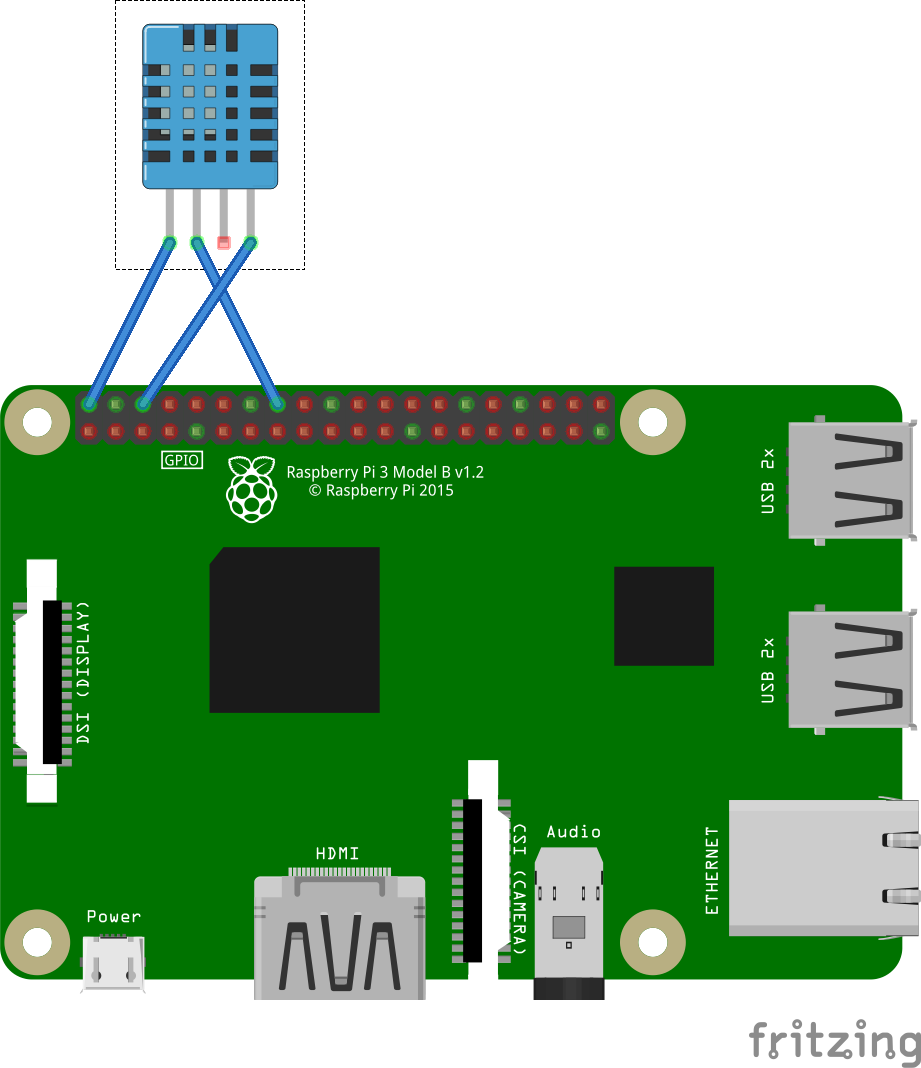
\includegraphics[width=0.6\paperwidth]{schema}}
            \caption{Esquemático para la conexión de la Raspberry Pi y el sensor.}
            \label{fig-schema}
        \end{figure}

        \paragraph{}
        En el repositorio de código comentado al inicio de esta sección, se encuentra el script en Python que debería ser ejecutado en la Raspberry Pi para que ésta lea los datos del sensor DHT11 y envié la información al MQTT Broker.

        \subsection{Virtualización de servicios}
        
        \paragraph{}
        Con el objetivo de automatizar las tareas de despliegue de toda la infraestructura desarrollada para el \textit{data pipeline} se ha optado por desarrollar la tecnología de virtualización Docker \cite{docker} junto con herramientas como Docker-compose \cite{docker-compose}. Todos los servicios han sido \textit{dockerizados}, es decir, incluidos en un contenedor que los aisla del resto. 

        \paragraph{}
        El uso de este tipo de tecnologías reduce de forma drástica el tiempo necesario para replicar el escenario desarrollado en distintas máquinas. Además ofrece ventajas para poder escalar cualquier tipo de recurso. Por ejemplo, el script que se utiliza para recoger la información de los sensores y enviarla al MQTT Broker puede ser incluido en un contenedor (con algunas modificaciones que simulen la lectura de datos desde los sensores) para tratar de mostrar el comportamiento que tendría el sistema al escalarlo a un entorno real.

        \paragraph{}
        Como se comenta en la sección de Diseño, el MQTT Broker y el Kafka cluster son elementos que no requieren ninguna personalización para nuestro escenario. Por tanto, podemos utilizar alguna implementación realizada previamente. Eclipse Mosquitto \cite{mosquitto} es una implementación del MQTT Broker ampliamente utilizada en despliegues de este tipo de tecnología. Para su inclusión, se ha utilzado la imagen oficial presente en el repositorio de imágenes de Docker \cite{mosquitto-docker}. Así mismo, existe diversas imágenes para el cluster de Kafka. En este caso, se ha optado por la opción cuyo soporte realiza Bitnami \cite{bitnami}, una compañía especializada en el soporte de este tipo de plataformas \cite{kafka-docker}.

        \paragraph{}
        Del mismo modo, las plataformas de la base de datos InfluxDB y el servicio que ofrece Grafana también pueden ser virtualizados con las imagenes oficiales desarrolladas por los desarrolladores de cada una de ellas \cite{influx-docker} \cite{grafana-docker}.

        \subsection{Desarrollo de servicios en Python}

        \paragraph{}
        Para la programación de todas las entidades que se han desarrollado se ha optado por desarrollar unos scripts básicos en Python que permitan simular el comportamiento que deben representar.

        \paragraph{}
        Para la utilización del protocolo MQTT en los distintos clientes se ha utilizado la librería \textit{paho-mqtt} \cite{paho-mqtt}, para el desarrollo del comportamiento del Kafka Producer y del Kafka Consumer se ha optado por utilizar la librería \textit{kafka-python} \cite{kafka-python} y para la funcionalidad relacionada con la gestión de la información en la base de datos InfluxDB se ha optado por la librería \textit{influxdb-python} \cite{influx-python}.
        
        \subsection{Análisis de datos} \label{sec-data-analysis}
        
        \paragraph{}
        Grafana es una herramienta que permite hacer cuadros de mandos de todo tipo. Desde cosas bastante sencillas a otras mucho más complejas. Para el alcance de este trabajo, se ha considerado interesante explorar las opciones que la plataforma ofrece realizando una aproximación a lo que podría ser un cuadro de mando que siriviese para monitorizar el estado de la temperatura en las distintas ubicaciones de lo Universidad de Murcia.

        \paragraph{}
        Para ello utilizaremos tres paneles que nos presentan la siguiente información:
        
        \begin{itemize}
            \item \textbf{Temperatura actual} en los distintas estancias utilizando un código de colores que permita conocer rápidamente el estado de los distintos edificios.
            \item \textbf{Evolución de la temperatura} en las distintas estancias en una ventana temporal que puede ser configurada como parámetro del cuadro de mando al que pertenece el panel.
            \item \textbf{Temperatura media} en la Universidad de Murcia. Es recomendable resaltar una medida que pueda ser utilizada como indicador clave (KPI) para medir el estado de un determinado elemento. En este caso, se ha seleccionado este valor de temperatura media que se resalta utilizando un código de colores igual que el de la temperatura actual para asociar el valor a un determinado estado.
        \end{itemize}

        \paragraph{}
        La figura \ref{fig-dashboard} muestra cómo puede verse este cuadro de mandos desarrollado y toda la información que ha sido comentada.

        \begin{figure}[ht]
            \centerline{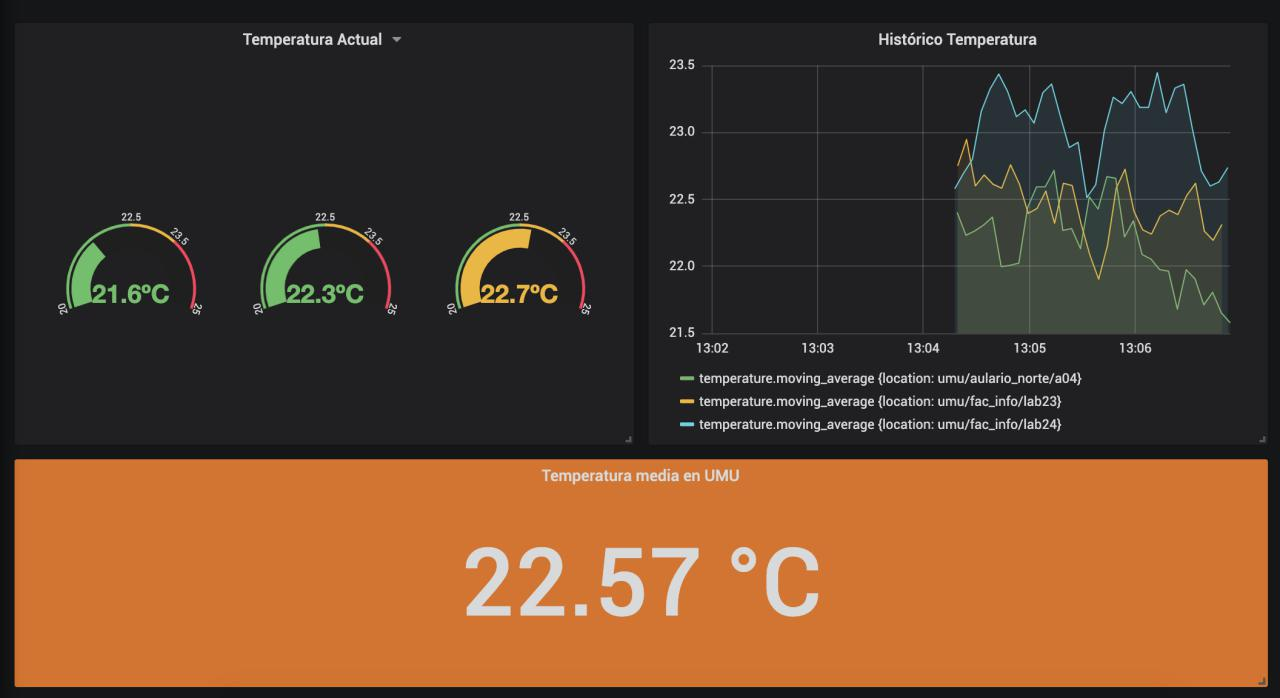
\includegraphics[width=0.8\paperwidth]{dashboard}}
            \caption{Dashboard en Grafana para analizar temperatura en la UMU.}
            \label{fig-dashboard}
        \end{figure}

        \section{Conclusiones}

        \paragraph{}
        Con este trabajo se ha conseguido construir un \textit{data pipeline} de forma completa que utiliza tecnologías que está siendo usadas en producción por grandes compañías. Además, ha cumplido con el objetivo de utilizar herramientas que no han sido utilizadas en ninguna de las asignaturas de la titulación.

        \paragraph{}
        Tras su realización, se propone como vías futuras para continuar con el mismo la profundización en todas las tecnologías que han sido utilizadas ya que su inclusión ha sido meramente simbólica y no se ha llegado a explorar con profundidad ni detenimiento de ninguna de ellas. Del mismo modo, sería interesante realizar un análisis de la idoneidad de este tipo de arquitecturas para algún escenario de despliegue real más allá del inventado para realizar las pruebas que permitiesen la elaboración de este trabajo.

        \paragraph{}
        Por otro lado, sería interesante destacar como la realización de este tipo de trabajos permite explorar tecnologías que quedan fuera del alcance de la programación de ninguna asignatura, permitiendo realizar un proceso de formación un tanto diferente al que se sigue tradicionalmente. Esto suele generar mucha contronversia en los alumnos puesto que tener que enfrentarse a trabajos con una temática libre es algo a lo que no se está aconstubmrado. No obstante, se deberían comenzar a valor de una forma mucho más positiva ya que implica el desarrollo de capacidades que no se suelen trabajar.

        \clearpage
        \addcontentsline{toc}{chapter}{Bibliografía}
        \bibliographystyle{plain}
        \bibliography{./memoria.bib}
    \end{document}